\chapter{MUSTANG}\label{chap:mustang}

{\bf NOTE: this chapter describes the use of MUSTANG, not of its
  successor MUSTANG-1.5 which will be installed on the GBT for
  commissioning and shared-risk science in early 2014. The use of
  MUSTANG-1.5 will be documented after commissioning is complete.}

MUSTANG (MUltiplexed SQUID TES Array at Ninety GHz), the GBT's first
3mm instrument, comprises a nearly fully-sampled array of 64
Transition-edge Superconducting (TES) bolometers which provide a $9''$
beam on the sky and instantaneously measure a $\sim 40'' \times 40''$
field-of-view.  It was built at the University of Pennsylvania by PI
Mark Devlin's group, in collaboration with NIST, NASA, NRAO, and
Cardiff University. It is now a facility instrument on the GBT.  This
chapter of the Observing Guide describes how to observe with MUSTANG
on the GBT.

%\htmladdnormallink{http://www.astro.umd.edu/$\sim$harris/kaband/\#guides}{http://www.astro.umd.edu/~harris/kaband/\#guides}

%++++++++++++++++++++++++++++++++++++++++++++++++++++++++++++++++++++++++++++
\section{Conditions Affecting MUSTANG Observations}\label{sec:mustangpreconditions}

This section outlines the factors which can affect the efficiency and
success of MUSTANG observations.

\subsection{Weather \& Solar Illumination}\label{sec:muswx}

Observations at 90 GHz are affected by clouds and water vapor, which
attenuate the astronomical signal and contribute spurious emission.
As a rule of thumb, data obtained with zenith 90 GHz sky brightnesses
(at zenith) under 35 K provide good data, and data obtained with 90 GHz sky
brightnesses under 50 K provide usable data for some of the easier
types of projects (compact or bright sources, for instance).  Due to
the fact that MUSTANG instantaneously samples many points on the sky,
and the GBT beams traverse nearly identical paths through the
atmosphere, the spurious emission contributed by the atmosphere can be
effectively removed by variants of a common-mode subtraction
implemented in the data reduction routines. The penalty which results
is that astronomical structures on scales much larger than one
instantaneous FOV are removed from the map. If the weather is clear
and stable, however, the common mode subtractions can be less
aggressive and larger structures can be reliably imaged. {\bf
\it The main effects of degraded weather will therefore be loss of
large-scale structure in the maps and further attenuation of the
astronomical signal}. In the case of poor weather (rain, heavy and
variable cloud cover) a large and variable attenuation can prevent
reliable flux calibration, so observing is not recommended.

A device measuring the net near-IR irradiance of the sky (called a
pyrgeometer) has been installed near the GBT and provides an approximate
indication of cloud cover. Its data are shown
on the {\tt GBTSTATUS} screen near the wind information.  Values more
negative than $-70 \, {\rm watts/m^2}$ indicate clear skies while
values more positive than $-15 \, {\rm watts/m^2}$ indicate thorough
cloud cover.

Wind and solar illumination affect the telescope structure and
therefore influence 90 GHz observations with the GBT as well.  Refer
to Chapter~\ref{chap:weather} for discussion of how weather affects
the GBT.  The effect of wind is somewhat less on MUSTANG observations
than for traditional targetted, single-beam, photometric observations:
since the sky is densely sampled and all observations are conducted
``on-the-fly'', one needs only to know where the beams were pointed at
a given time rather than to keep the telescope pointed accurately at a
given spot. A ``quadrant detector'' on the GBT helps to increase the
accuracy of this reconstruction on the GBT and the data from it is
automatically used by analysis algorithms.  {\bf \it A good rule is to
only use data from scans with mean winds under 10 mph and peak winds
under 12 mph}.  There are three GB weather stations, and to be
conservative, use the maximum of the readings of the operable weather
stations at a given time. The data reduction tools described in
\S~\ref{sec:musdatareduc} provide this information on a scan-by-scan
basis during or after the observations. Conditions can also be
monitored in the GBTSTATUS tab of astrid and in various CLEO screens
(principally the weather and status screens).

The Dynamic Scheduling System (DSS) will schedule MUSTANG proposals when the 
forecasted winds are $\leq 10mph$, opacities are reasonable ($\leq\sim 0.25$) and cloud
cover is sufficiently low.

\subsection{Source Elevation}\label{sec:mussrcvis}

Several considerations constrain the range of elevations at which
useful MUSTANG observations can be conducted: the atmospheric opacity,
typically $0.07 < \tau_{90 \, GHz} < 0.15$ per airmass in useful
observing conditions, which attenuates the astronomical signal at low
elevations; the MUSTANG cryogenics, which do not operate effectively
below 19 degrees elevation; microphonics from other receivers, which
couple more strongly at lower elevations; and the antenna primary
surface, which shows a constant 90 GHz gain between 20 and 80 degrees
elevation but can drop off sharply outside of this range. Putting
these considerations together and summarizing:
\begin{itemize}
\item elevations below 20 degrees: not recommended due to reduced 
telescope gain and severely degraded MUSTANG cryogenic performance.
\item 20 - 30 degrees elevation: usable performance for observations of
bright sources. Receiver noise can be several times higher due to
microphonics and the astronomical signal will be attenuated by a factor
of 2 to 3 more than at zenith.
\item 30 - 80 degrees elevation: good performance. Within this range,
the optimal performance is seen between 50 and 65 degrees elevation.
\item above 80 degrees elevation: not recommended. Photometric
performance in this range is not consistent, probably due to
degradation of the primary surface model. Above 85 degrees the antenna
often fails to execute MUSTANG scan trajectories due to the rapid slew
rates in azimuth that are required for an Alt-Az telescope such as the
GBT to track close to the zenith.
\end{itemize}

\subsection{Receiver Cryogenic State}\label{sec:musrcvrvis}

The receiver should be cold and stable before observations begin.
Whether or not this is the case can be determined by inspecting the
MUSTANG CLEO screen (see Section~\ref{sec:cleo}).  The detector array (``array G0'') should be
under 400 milliKelvin and shouldn't be changing by more than a
milliKelvin or two per reading (there is one reading every few
minutes); the series array should be under 5 Kelvin.  The bolometer
array is kept cold by a closed-cycle helium fridge, consisting of two
separate, closed ``pots'': one with liquid He3 and one with liquid
He4. The liquid in these pots boils away, thereby cooling the
detectors, and is captured internally; when it has all boiled away it
must be re-condensed or ``cycled''. The MUSTANG CLEO screens present
conservative estimates of how much time remains for the He3 and He4
fridges. Ideally there will be enough of both to cover your entire
observing run.  Only He3 is required to operate MUSTANG, although if
He4 runs out in the middle of a run the detectors will warm up
slightly and need to be re-biased (\S~\ref{sec:mussetup}).

Observatory staff are responsible for delivering appropriate cryogenic
conditions but due to external factors it will occasionally not be
possible at the start of a run. If this has occured the operator or
support scientist will inform you of the situation and recommend a
course of action.  Time lost to cryogenic failures, like other
lost time from hardware failures, will not be charged to the balance of your project
time.

\section{Preparing for, and Cleaning up after, Observations}\label{sec:mussetup}

Your GBT friend or support staff will have MUSTANG tuned up and ready
to go at the start of your run. These settings should have been saved
to

\noindent
{\tt /home/gbt/etc/config/mustang\_config/current.conf}

From a terminal(s) on a 32-bit machine on the gbt network:
\begin{itemize}

\item As for other GBT observations, start {\tt ASTRID} and {\tt CLEO}. Within {\tt CLEO},
select {\tt Launch} $\rightarrow$ {\tt Receivers} $\rightarrow$ {\tt
MUSTANG}.The housekeeping tab is most useful to have up during
observations.

\item Start the MUSTANG data monitor. To do this first

\noindent
{\tt source /home/gbt/gbt.bash}

\noindent
(or source gbt.csh if using C-shell). Then type

\noindent
{\tt mustangdm}

\item Run the {\tt mustanginit} scheduling block (SB). This scheduling block sets up ASTRID and
performs basic initialization of MUSTANG.

\item Run the {\tt TweakTargets} and {\tt FindBestBiases} SBs, in that order. These
SB's find and set usable detector biases and optimize the SQUID
tuning; they will require about 5 minutes to execute.

\item Run {\tt savetuning} SB. This will save the tunings so that they can be
restored, if needed, later.

%\item Run the {\tt recordsquidcalib} SB, which will take 30 seconds. This collects
%a short datafile documenting the instrument calibration state.

\item Collect a cal file to check that everything is in working order using
the {\tt calandblank} SB.  This will collect two scans, one with the
cal diode flashing on and off to check for optical responsivity, and
one file with the cal off the check detector noise.

\item Fire up the MUSTANGIDL GUI and check the cal data as described in \S~\ref{sec:musdatareduc}

\item Proceed with observing, as described in \S~\ref{sec:musobsstrat}.

\end{itemize}

As the last scheduling block (SB) in your program please run {\tt
mustangshutdown} to leave the receiver in a quiescent state.


%%%%%%%%%%%%%%%%%%%%%%

\section{Observing with MUSTANG}\label{sec:musobsstrat}



\subsection{Mapping Strategies}\label{sec:musmap}

All MUSTANG data are collected with variants of an ``on-the-fly''
(OTF) mapping strategy in which the antenna is slewed to cover a given
region of interest while data are recorded.  Two main scan strategies
have been developed: a ``box'' or ``billiard-ball'' scan which covers
a rectangular region with approximately uniform coverage; and a
``daisy'' or ``spirograph'' scan pattern which covers a circular area
with a more center-weighted distribution of integration time on the
sky. Under normal circumstances we do not recommend the standard
ASTRID observing procedures RALONGMAP or DECLATMAP which perform
discrete, linear raster-scans over a given region because these tend
to excite vibrations of the GBT feedarm which in turn give rise to
unacceptable pointing errors at 90 GHz. Due to the desirability of
covering a given point of interest on the sky with many detectors, and
due to the effects of fluctuations in detector gain and sky noise, we
do not recommend staring at a single point either, even for
point-source photometry projects. Under these circumstances the
center-weighted coverage of the daisy scan is appropriate. For the
identical total integration times and areas covered the daisy pattern
gives a factor of $\sim 3.6$ more integration time on the central
field-of-view, or a reduction of $\sim 1.9$ in RMS noise compared to
uniformly distributed integration.


The daisy scan pattern is supported by ASTRID directly and can
be invoked as follows:
\begin{lstlisting}
Daisy('1331+3030',daisyRadius,daisyRadialPeriod,0,0,scanDuration, \
       beamName='C')
\end{lstlisting}
where
\begin{itemize}
\item daisyRadius is the radius of the circular area to be covered, in arcminutes
\item daisyRadialPeriod is the period of radial oscillations, in seconds (not to be less than 15 sec $\times 
\sqrt{daisyRadius/1.5 \,arcmin}$ for radii $>1.5'$ and in no case under 15 seconds).
\item scanDuration is the scan duration in seconds. Approximately 22 radial periods are required to completely
cover a circular area with the default parameters.
(Also see notes in section~\ref{sec:notesdaisy}).
\item beamName must be 'C' for MUSTANG since individual beam offsets are not defined in the antenna
database.
\end{itemize}
An example trajectory is shown in Figure~\ref{fig:daisytraj}. For
photometry of point sources you want the array at some point to be
completely off source ($r\sim 0'.8$). Typical radii are $1'$ to $5'$.

\begin{figure}
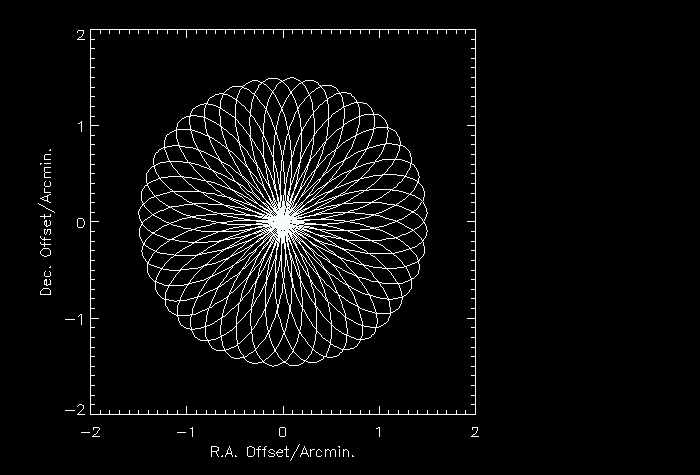
\includegraphics[width=4.5in,bb=0 0 700 475]{daisytraj.png}
\caption{Full (22-cycle) daisy scan trajectory with a radius $r=1'.5$.}
\label{fig:daisytraj}
\end{figure}

To cover rectangular areas more uniformly there is a custom ``Box'' scan procedure, invoked
as follows:
\begin{lstlisting}
DefineScan("boxtraj", "/users/bmason/gbt-dev/scanning/ptcsTraj/boxtraj.py")
boxtraj(mySrc,x0=x0,y0=y0,taux=taux,tauy=tauy,scanDuration=scandur, \
        dx=dx,dy=dy)
\end{lstlisting}
where
\begin{itemize}
\item x0 and y0 specify the box width and height in arcmin
\item taux and tauy specify the periods of motion in either direction, in seconds
\item scanDuration specifies the scan duration in seconds
\item dx and dy specify dither offsets for the trajectory in arcminutes. In practice
a $2/3$ beam ($6''$) triangular dither serves well.
\end{itemize}
{\tt boxtraj} executes a truncated sawtooth waveform in each direction (RA and Dec, typically) with 
specificable periods taux and tauy. Combinations of (taux,tauy,x0,y0,scanDuration) which give approximately
uniform coverage have been determined by experimenting with simulations. Some common ones which
also comply with GBT motion limitations are:
\begin{itemize}
\item $2' \times 2'$ to $3' \times 3'$, square patterns, are well covered by taux=10 sec, tauy=8 sec,
and a 160 second total scan duration.
\item $5' \times 5'$ to $7' \times 7'$ square patterns are well covered by taux=9, tauy=8, and a total
scan duration of 290 seconds.
\end{itemize}
An example box scan trajectory is shown in
Figure~\ref{fig:boxtraj}. If the area to be covered is substantially
larger than any of these regions and not suitable to be covered by
tiling, your staff friend can help find suitable parameters.

\begin{figure}
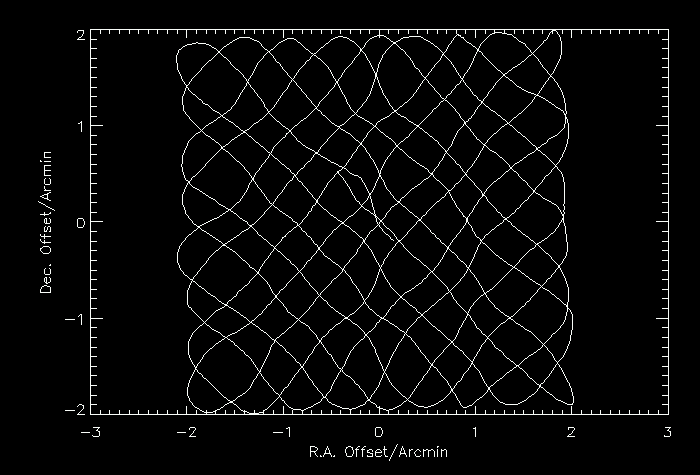
\includegraphics[width=4.5in,bb=0 0 700 475]{boxtraj.png}
\caption{$4'$ box scan trajectory.}
\label{fig:boxtraj}
\end{figure}


\subsection{Sensitivity}

When mapping a $3' \times 3'$ region uniformly (i.e., with a box-scan
approach) MUSTANG typically achieves a map noise of $0.4 \, {\rm
mJy/beam}$ (RMS) in one hour of integration time.  This RMS descreases
as $\sqrt{t}$ for many hours under good conditions, and (for a fixed
integration time) increases as the area covered for larger
areas. Gains cannot be made by covering smaller areas uniformly due to
practical limitations associated with the telescope motion and
detector noise characteristics. However, for photometry of point or
compact sources, the daisy scan will deliver a factor of $1.9$
improvement in RMS for a fixed integration time ($0.2 \, {\rm
mJy/beam}$ RMS in one hour integration, for the central $d=1'$ area
covered).

\subsection{Establishing \& Monitoring Good 3mm Performance of the Antenna}\label{sec:musgbt}

It is imperative to establish good 90 GHz performance of the GBT at
the start of your observing run and monitor it carefully
throughout. This entails determining any corrections to the GBT
subreflector focus position that are needed, and determining any
corrections for thermal deformation of the GBT surface that are
needed.  To do this we use the technique of Out-of-Focus (or phase
retrieval) Holography, also known as OOF. The phase retrieval
technique uses data from a series (typically three) of beammaps
collected at different focus settings to reconstruct low-order phase
errors at the dish surface, which can then be corrected with the GBT's
active surface. The same data are used to derive a consistent set of
corrections to telescope pointing and focus, which are also applied
online via the telescope control system.  The {\tt ASTRID} {\tt
AutoOOF()} procedure will acquire and analyze these data and give you
the option to send them to the telescope. Acquiring the OOF data
should take about seven minutes; analyzing them will take another five
to seven.  When complete, send the surface correction to the telescope
from the AUTOOOF tab and collect a single in focus scan to verify that
the beam shape is still reasonable (not larger than before!) and that
the source amplitude is equal to or greater than what was seen before
the surface correction was sent.  If the data pass these sanity
checks, you are ready to proceed to your science observing. Otherwise,
repeat the focus and/or primary surface measurement. The {\tt AUTOOOF()}
procedure also determines and applies subreflector focus and
pointing corrections.

{\bf Note:} once the processing is complete, it is the {\it first}
``Send Solutions'' button (marked ``new, recommended method'') that
you want to push to send the surace, pointing, and focus corrections
to the telescope. If you push the second (``old, original'') button the
focus offset will not be sent, which may result in irretrievable
degradation of the quality of your data.

You can also manually check the focus with a more fully sampled series
of maps (typically five) collected at a range of focus positions. The
{\tt parFocusDaisies} example scheduling block implements such a
measurement, which can be analyzed as described in
\S~\ref{sec:musdatareduc}. We recommend you only take this approach
if you have reason to doubt the corrections derived by {\tt AutoOOF}
-- for instance, the peak source intensity obtained after applying the
focus and pointing solutions from {\tt AutoOOF} is lower than the peak
source intensity before. {\bf Note:} {\tt parFocusDaisies} centers the
focus scans on the focus correction value (LFCY) set by the variable
{\bf nomfocus}, and leaves it at this value at the end! Do not forget
to set nomfocus to the current local focus Y-correction (LFCY) before
running it. After running {\tt parFocusDaisies} and analyzing the
data, you can send the pointing (in arc{\it minutes}) and focus
corrections (in millimeters) either by telling them to the operator or
by editing and running the example {\tt applyptg} SB.

Every half hour you should check the focus and beam shape by obtaining
a single quick map (SB {\tt quickdaisy}) of a calibrator source,
monitoring the beam size, pointing, and relative source amplitude over
time. At this time, another {\tt calandblank} should also be done.  If
the beam size increases by more than 10\%, or the source amplitude
decreases systematically by 15\% or more, then it is likely that the
thermal corrections to the GBT primary and/or the subreflector focus
corrections need updating, and it is time to do another AUTOOOF.
(note: beam size and source amplitude degradation may also be caused
by poor weather). While the AUTOOOF procedure will update the
telescope pointing corrections as well, it is not necessary to perform
an AUTOOOF just to correct pointing which has drifted assuming the
beam shape and source amplitude are stable.  The pointing offsets can
be corrected after the fact in the data analysis using your periodic
calibrator monitoring observations.

\subsection{Calibration}\label{sec:muscalib}

{\it It is essential to observe a flux calibrator during each
observing session, and to do this only after the initial set of active
surface (OOF) corrections have been applied}. Changes in gain due to
subsequent OOF corrections if any can be tracked with the secondary
calibrator. The recommended MUSTANG flux density scale is ultimately
based on the WMAP 7-year (Wieland et al. 2010) measurement of Mars,
however, Mars is often not visible and is resolved by the GBT at 90
GHz, complicating its use. A list of secondary flux calibrators
sufficiently compact and stable (or have modelable light curves) is
shown in Table~\ref{tbl:musfluxcals}.  Other sources may also be
suitable given appropriate bootstrapping observations.  Custom
ephemeris can be obtained from the JPL online {\tt HORIZONS} system
and translated into the {\tt ASTRID} format. Work is under way
to increase the number of secondary (bootstrapped from planets)
flux calibrators.

\begin{table}
\begin{tabular}{|l|l|l|l|}
\hline
Name & R.A. (J2000) & Dec. (J2000) & Notes \\ \hline
Uranus & 0h & 0d & In ASTRID  \\
Neptune & 22h & -12d & In ASTRID \\
Mars & 13h-24h & -10d & In ASTRID; extended \\
Saturn & 12h & 0d & In ASTRID; extended \\
Ceres  & 17h - 22h & -20d & Use custom ephemeris\\
W3(OH) & $02:27:03.8$ & $+61:52:24.8$ & extended \\
Mwc349 & $20:32:45.6$ & $+40:39:37$ & -\\
CRL2688& $21:02:18.8$ & $+36:41:37.8$ & slightly extended \\ \hline
\end{tabular}
\caption[A list of secondary flux calibrators suitable for use with MUSTANG]
{A list of secondary flux calibrators suitable for use with MUSTANG.
Coordinate ranges are for the 2010/2011 observing season.}
\label{tbl:musfluxcals}
\end{table}

A catalog of 27 compact, 90 GHz bright sources is at {\tt
/users/bmason/mustangPub/mustangpnt.cat}. These sources are suitable for
peak/focus/OOF check observations and for monitoring the antenna
performance, but are {\it not} suitable for flux calibration.

\subsection{Observing Summary: Example Observing Sequence}

An example observing sequence would be as follows:
\begin{itemize}
\item mustanginit
\item TweakTargets \& FindBestBiases
\item savetuning
\item calandblank
\item on a 1 Jy or brighter point source--
\begin{itemize}
\item quickdaisy: check the gain and beam size on a calibrator
\item autooof: establish GBT surface corrections
\item quickdaisy: check gain and beam size after applying surface corrections
\end{itemize}
\item quick daisy on primary flux calibrator. if this is a large slew (over 60 degrees in az, over 30 degrees
in el) you might want to run focus daisies centered on the current LFCY just to be safe.
\item quick daisy on secondary flux calibrator within 15 degrees of science target. if this is a large slew you might want to run focus daisies centered on the current LFCY just to be safe.
\item half hour of observing (boxmap or parfulldaisy)
\item quickdaisy on nearby secondary (pointing/focus) calibrator. If the beam gain has gone down by 15\% or more, or the beam become 10\%
fatter in one or both directions, repeat an AutoOOF on the pointing calibrator, and verify results with a quickdaisy.\item calandblank
\item half hour of observing (boxmap or parfulldaisy)
\item quickdaisy to check gain and focus
\item calandblank
\item {\it et cetera}.
\item mustangshutdown
\end{itemize}

\section{Quick Look Data Reduction}\label{sec:musdatareduc}

It is essential to monitor the quality of your data as you are
collecting it. A suite of tools has been written in IDL to make this
possible. This section outlines its use.  {\it \bf We highly recommend
that you reduce your imaging data as you go along so that you can
catch problems should they develop}.

For monitoring ongoing observations, observers should use the GUI interface
to the MUSTANG IDL code. This can be started from the UNIX command line
on any Green Bank UNIX machine as follows:
\begin{lstlisting}
[username@prospero]~bmason/mustangPub/mustangidlgui
\end{lstlisting}

The first step is to select the project you are working with via the
``Browse Projects'' button; selecting ``Online'' will select the most
recently updated project in /home/gbtdata (probably your project, if
you are observing on the GBT). You can also, for inspection of
already-acquired data, type in the full path to the data directory in
the box (for instance, /home/gbtdata/AGBT11C\_033/ or
/home/archive/science-data/tape-030/AGBT07B\_012/ -- note the trailing
slash).  Once this is done the area at the bottom of the GUI will
display a summary of your telescope period so far. This summary can be
updated with the ``Update Scan Summary''.  At this point IDL will
read all files in the project directory so far and generate a summary
(in the GUI window, and also in the terminal window the IDL GUI was
launched from):
\begin{lstlisting}
IDL> summarizeparproj
#                                         Scan#/                           
# Scan       File name          ScanType  out of       SB       SrcName     
   1 2009_02_21_07:35:25.fits     Track    1 / 1  calandblank     cal      
   2 2009_02_21_07:35:49.fits     Track    1 / 1  calandblank     Blank    ...
   3 2009_02_21_07:52:30.fits    RALongMap 1 / 1     focus       1337-1257 
   4 2009_02_21_07:53:28.fits    RALongMap 1 / 1     focus       1337-1257 
\end{lstlisting}
The GUI will also now have a list of valid ``CAL'' scans in the drop
down CAL SCAN box (see below).


There are some latencies involved in getting all the FITS files
written to disk so the current scan may not be accurately reflected in
the summary. For this reason you should also not try to make a map
with the current scan -- wait about 1 minute after the completion of a
scan to try and map it. We tried to make the IDL code as robust as
possible but this will sometimes crash the code. In this event restart
the IDL gui, re-enter the proejct (or click online) and re-select the
cal scan you dsire. 

\begin{figure}
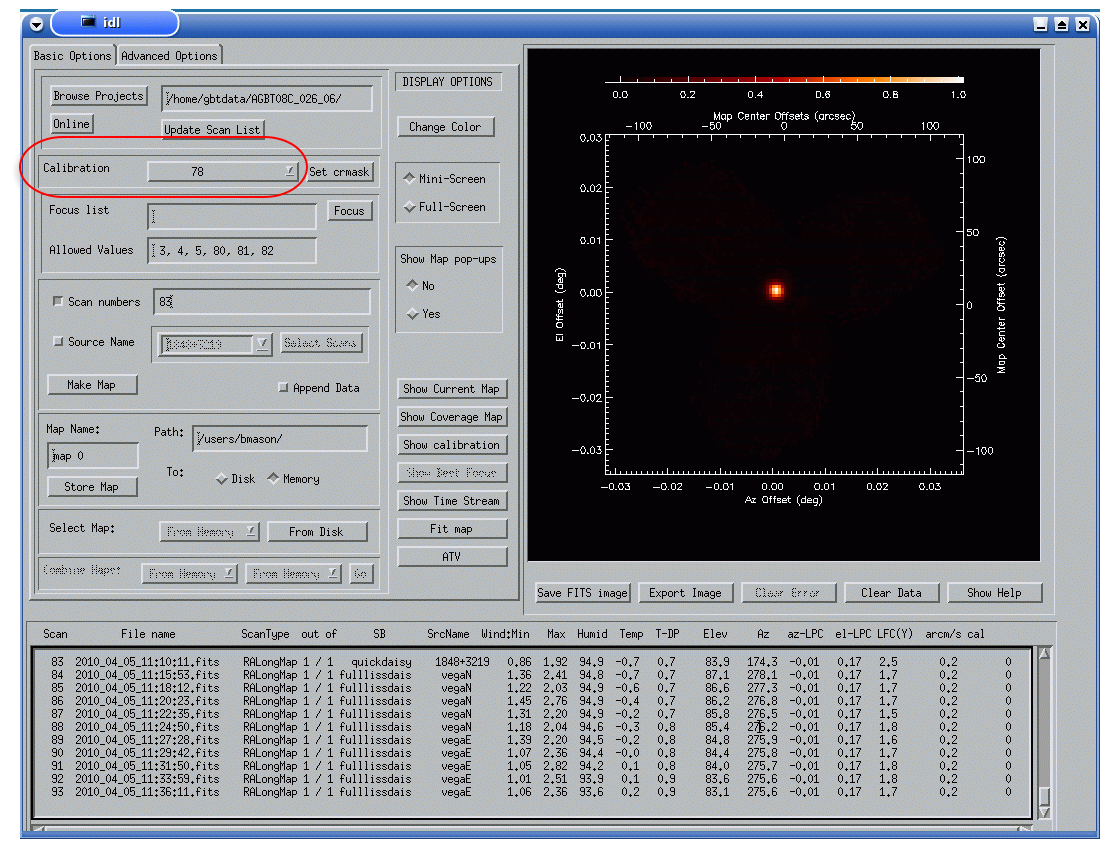
\includegraphics[width=4.5in,bb=0 0 1109 848]{mustangGuiCalib.png}
\caption{Selecting the CAL scan in the MUSTANG IDL GUI.}
\label{fig:calgui}
\end{figure}

The relative pixel gains are calibrated by flashing an internal cal lamp on and
off, done by the {\tt calandblank} SB. The data from a CAL scan are analyzed by
selecting the desired scan in the drop down box in the GUI (see Figure~\ref{fig:calgui}).  Partial example output
is as follows:
\begin{lstlisting}
docalib,calscan=1,gain=mygain,crmask=mycrmask
.
.
.
 *** GAINS: 
 -1.18084e-12    0.0688694      155.829      200.706  
      0.00000     -93.2362      83.6297      148.163  
 -1.18084e-12     0.320343      101.007      298.489  
      0.00000     -77.4885      141.224      184.050  .....
      0.00000     -81.9272      79.5458      107.280  
      0.00000     -82.3489      92.1591   -0.0603582  
      0.00000     -57.1215      73.7274      148.184  
      0.00000     -59.1193      73.8523      313.731  
      0.00000  0.000713527   -0.0108514   -0.0494373  
 *** CRMASK and total:       49.0000
      0.00000      0.00000      1.00000      1.00000    
      0.00000      1.00000      1.00000      1.00000    
      0.00000      0.00000      1.00000      1.00000    
      0.00000      1.00000      1.00000      1.00000    
      0.00000      1.00000      1.00000      1.00000    .....
      0.00000      1.00000      1.00000      0.00000    
      0.00000      1.00000      1.00000      1.00000    
      0.00000      1.00000      1.00000      1.00000    
      0.00000      0.00000      0.00000      0.00000    
\end{lstlisting}
The top shows the gain (in nominal counts per Jansky) and the bottom
shows the ``column-row'' mask denoting optically responsive detectors
with ``1'' and optically non-responsive detectors (or those flagged by
automated criteria) by ``0''. The pixel gains serve the purpose of
flat-fielding the detectors but the flux density scale is fiducial
only and celestial calibration is still essential. The routine
summarizes its findings in the above form, organized by logical row
and column ({\it i.e.}, electrical labels for each detector rather
than array-face geometry). In this case all of column zero is
non-responsive and only four columns are shown due to space
limitations.  Row 8 (zero indexed) is always non-responsive since this
is by design each column's dark SQUID, not connected to a bolometer.

Given a nominal detector calibration, mapping data can be made into
images by entering the desired scans in the box labelled ``Scan
Numbers'' and clicking ``Make Map'' (see Figure~\ref{fig:mapgui}).
This uses the default imaging parameters, which should be suitable for
most situations but which can be changed in the ``Advanced'' tab. The
coverage map can also be displayed by clicking the ``Show Coverage
Map'' button; this results in an image of weight per pixel (units of
inverse Janskys squared) and is approximately proprtional to
integration time, and inversely proportional to map noise variance.
The map can be saved to a FITS file by clicking on ``Save FITS
Image''. These files can be manipulated by standard astronomy imaging
packages ({\it e.g.}, {\tt ds9}, {\tt fv}).

\begin{figure}
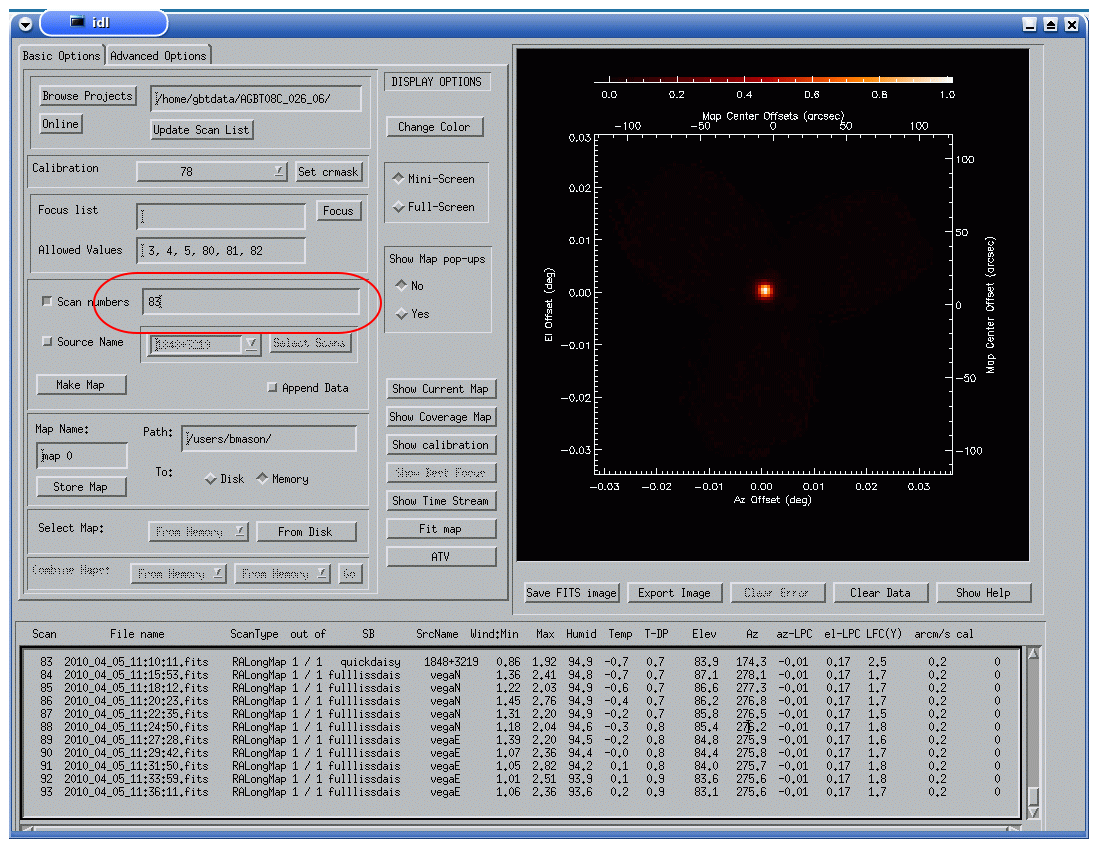
\includegraphics[width=4.5in,bb=0 0 1098 848]{mustangGuieScanNumbers.png}
\caption{Specifying scans to image in the MUSTANG IDL GUI.}
\label{fig:mapgui}
\end{figure}

For monitoring the amplitude and beam-width of the twice-hourly
pointing calibrator observations, the GUI provides the facility to fit
each map to a Gaussian. To reduce the calibrator observations you can
use the default (Right Ascencion/Declination) coordinate system but it
is often more useful to make the map in Elevation/Cross-Elevation
coordinates (i.e., offset relative to the source nominal ``True''
position) in order to monitor the telescope pointing offset.
This can be done by selecting ``EL/XEL'' coordinates in the ``Advanced''
tab (see Figure~\ref{fig:elxel}). A given map can be fit to a Gaussian with the ``Fit Map'' button;
the amplitude and beam width (FWHM) are shown in the terminal
window and the GUI text output window. Since an elliptical Gaussian
is used, there are two parameters for the width.

\begin{figure}
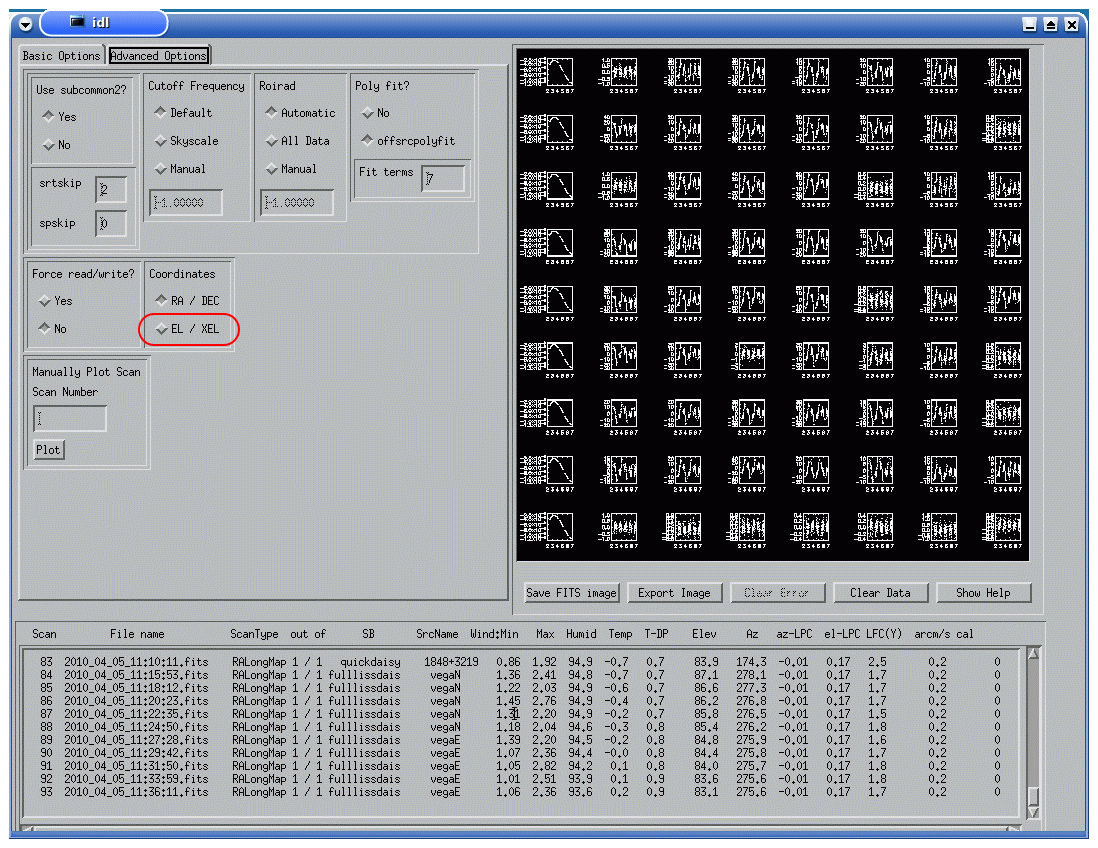
\includegraphics[width=4.5in,bb=0 0 1098 848]{mustangGuiElXel.png}
\caption{Specifying the coordinate system for the maps in MUSTANG IDL GUI.}
\label{fig:elxel}
\end{figure}

The imaging routines produce diagnostic feedback primarily intended
for support staff. Many IDL routines also produce a floating point
exception which can be safely ignored.

In the unlikely event that the beam degrades, {\tt AutoOOF} does not
fix it, and you have acquired {\tt parFocusDaisies} data to check it,
you may enter the scan numbers of the focus maps in the ``Focus list''
box. Each scan will be imaged and fit to a Gaussian, and the beam
width and amplitude as a function of focus offset (LFC) will be
plotted.  Choose the LFC that minimizes the beamwidth and maximizes
the source response and enter this into the Antenna Manager CLEO
screen, or have the operator do so.  The amplitude does not always
peak at the same focus position that minimizes the beam shape, but it
should be within a few millimeters.  Choose a focus position that for
your purposes is a good compromise between these two. In the lower
(beam width or FWHM) plot, the two widths are represented by a dot and
a diamond. Therefore a circular beam, which is a good indication of
being in focus, will correspond to the dot and the diamond coinciding.
This is illustrated in Figure~\ref{fig:musfocus}.

{\bf \it When processing focus data, note that it can often take up to
a minute for the most recently completed scan to become readable on
the filesystem}, so exercise some patience when processing your data
on-line. 

\begin{figure}
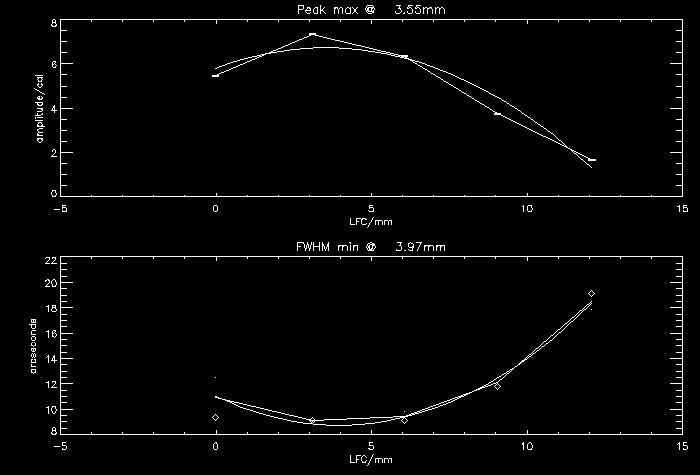
\includegraphics[width=5in,bb=0 0 700 475]{betterfocus.png}
\caption[Summary plot produced by best\_focus showing an optimum
value for LFC\_Y]
{Summary plot produced by {\tt best\_focus} showing an optimum
value for {\tt LFC\_Y} of about $3.7 \, {\rm mm}$.}
\label{fig:musfocus}
\end{figure}

You can see the current LFCY in the ASTRID ``GbgStatus'' tab in the
entry labeled ``LFC (XYZ mm):'' --- it is the second number of the
three.

\section{Troubleshooting}\label{sec:musproblems}

GBT 90 GHz observing requires
diligence on the part of the observer. Following are some problems
that can come up, their symptoms, and first actions to take in
response:
\begin{itemize}

\item {\it GBT out of focus}: the beam gets larger and the peak gain lower than it had been before.
Check and reset the telescope focus.

\item {\it GBT primary deforms} due to changing structure temperatures: after
optimizing the focus the in-focus beam is still larger or lower-gain than
before. Rerun {\tt AutoOOF}.

\item {\it Detectors reach the edge of their dynamic range}: DAC values in
mustang monitor reach 0 or 16384. run a {\tt calandblank}, which
relocks the detectors mid-scale, or relock manually in the MUSTANG
{\tt CLEO} screen (column control tab).

\item A {\it greatly diminished cal or source response, or greatly diminished number
of live detectors}, can occur if the He4 runs out and the detectors
warm up a little.  With Helium-3 and Helium-4 both the Array G0
(detector array) temperature should read about 300 mK when detector
biases have been applied for a few minutes; with only Helium-3 it will
read about 340 mK with biases. Recondensing the He4 requires $1.5$
hours and puts the instrument out of use for that time; it is possible
to observe without, provided new biases are obtained (support staff
can help with this). If the He3 has run out it must be recondensed.

\item The MUSTANG IDL pipeline has an automatic binary cache mechanism which
greatly speeds up processing of a given scan after the first time it has been read. 
Unfortunately if the first reading of a scan was messed up for some transient
reason the binary cached version can get messed up. If the data are strange or
repeatedly unprocessable, try including the {\tt forceread} or {\tt focewrite}
options in analysis routines such as {\tt multimakemap} or {\tt best\_focus}.

\item {\it Data Latencies Crash IDL}: as previously noted, it sometimes takes 10s of seconds
for the data files to be complete and visible on disk to IDL. Trying
to read the latest scan too soon can result in IDL crashing.  In this
case, restart the IDL gui, reselect your project (or click ``online''
if you are observing, which will automatically select the most recent
telescope period with data); reselect the cal scan; and proceed.

\end{itemize}

\newpage

\section{Example ASTRID Scripts}\label{sec:musastridscripts}

The following sub-sections present some template ASTRID scheduling
blocks (SB's).  Templates are also kept in ASCII format in {\tt
/users/bmason/mustangPub/sb/}.  {\bf Note: the SBs in this document
are for the sake of example only; use the template SBs in the above
UNIX file path to get the latest version}.

\subsection{mustanginit}
\begin{lstlisting}

Configure("/users/bmason/mustangPub/sb/mustangfull.conf")

\end{lstlisting}

\subsection{autooof}

\begin{lstlisting}
mySrc=''1159+2914'
Catalog()
Slew(mySrc)
AutoOOF(source=mySrc)
\end{lstlisting}


\subsection{calandblank}

This SB runs a 15 second scan with the cal diode firing on and off,
allowing the bolometer responsivities to be measured, and a 30 second
scan tracking blank sky, allowing a check on the detector noise.

\begin{lstlisting}

# duration of cal and blank scans
#  in seconds
calduration=15
blankduration=30

# uncomment these 3 lines
#  to do the calibration at a given
#  az/el
# myAz=260
# myEl=78
# myLoc=Location("Encoder",myAz,myEl)
# or use this one to use the current az/el
myLoc=GetCurrentLocation("Encoder")

# do not modify from here down
#  extra information (source names, caltags etc)
#  is added for the sake of data analysis software,
#  which depends on these tags.
############

Slew(myLoc)
Configure("/users/bmason/mustangPub/sb/mustang.conf")
execfile("/users/bmason/mustangPub/ygor/relockAstrid.py")
Configure("/users/bmason/mustangPub/sb/calon.conf")
Annotation("CALTAG","DIODE")
SetValues("ScanCoordinator",{"source":"cal"})
Track(myLoc,None,calduration)
Configure("""
mustang.init='cal'
swmode='tp_nocal'
tint=0.001
""")
Annotation("CALTAG","BLANK")
SetValues("ScanCoordinator",{"source":"Blank"})
Track(myLoc,None,blankduration)
Annotation("CALTAG")
SetValues("ScanCoordinator",{"source":"nothing"})
Configure("/users/bmason/mustangPub/sb/caloff.conf")
\end{lstlisting}

\subsection{parFocusDaisies}

This SB runs a sequence of five maps at a range of subreflector focus
settings about the nominal focus. {\bf \it The nominal focus is in the
script as the variable {\tt nomFocus}; you should set it to the current
best-determined focus setting, and remember that the script will leave
it at that value upon completion}. Each map takes 45 seconds; the total
SB should run in about 5 minutes.

\begin{lstlisting}

# some good sources are...
# 1642+3948; 2253+1608; 0927+3902, 0319+4130
#  0359+5057. 1955+5131, 1256-0547
# 0854+2006
mySrc="1415+1320"

#################################
# CATALOGS
# none needed for planets

Catalog()

Configure("/users/bmason/mustangPub/sb/mustang.conf")

#################################
# start, stop, and increment for focus,
#  in mm
#
# current, nominal LFC
nomFocus=0
# LFC deltas to try around this
dfocus=(-10,-3,0,3,10)
# focus is left at nomFocus

#################################
#  Daisy Params
#
daisyScanDur=45.0
daisyRad=1.5
daisyRadPd=15.0

#######################################################
#######################################################
# Do not modify below here
#


from time import sleep

Slew(mySrc)							       
Configure("/users/bmason/mustangPub/sb/mustang.conf")

# relock MUX
execfile("/users/bmason/mustangPub/ygor/relockAstrid.py")

for df in dfocus:
    # set focus
    ff=df+nomFocus
    SetValues("Antenna",{'local_focus_correction,Y':ff})
    SetValues("Antenna",{"state":"prepare"})
    sleep(3)
    Daisy(mySrc,daisyRad,daisyRadPd,0,0,daisyScanDur,\
          beamName='C',cos_v=True,coordMode="Encoder",calc_dt=0.2)

#
# leave in nominal state
SetValues("Antenna",{'local_focus_correction,Y':nomFocus})
SetValues("Antenna",{"state":"prepare"})

\end{lstlisting}

\subsection{applyptg}

This SB applies pointing and focus offsets to the telescope. The
desired focus offset in millimeters is set in the python variable {\tt
focusoff}. Typically it is not necessary to do this by hand any more,
as the {\tt autooof} procedure takes care of the pointing and focus
offsets in addition to the surface.

\begin{lstlisting}

myLoc=GetCurrentLocation("Encoder")
# offsetts to apply in arcmin - LEAVE AT ZERO
azoff=0
eloff= 0
# Y focus offset in mm
focusoff=-3

#############################

azoff=azoff/60.0*3.14159265/180.0
eloff=eloff/60.0*3.14159265/180.0
SetValues("Antenna",{'localPointingOffsets,azOffset2':azoff})
SetValues("Antenna",{'localPointingOffsets,elOffset':eloff})
SetValues("Antenna",{'local_focus_correction,Y':focusoff})

\end{lstlisting}


\subsection{quickdaisy}

{\tt quickdaisy} collects a single quick map using the daisy scan
pattern. This is useful, for instance, to check your calibration every
half hour. It's not a bad idea to do two of these back to back, since
they each take less than a minute, which will also give you a check of
the photometric accuracy of your measurements every half hour.

\begin{lstlisting}

# some good sources are...
# 1642+3948; 2253+1608; 0927+3902, 0319+4130, 0854+2006
mySrc= "Ceres"

Catalog("/users/bmason/gbt-obs/par/ceres.ephem")

#################################
# CATALOGS
# none needed for planets
#
# standard pointing source catalog :
#      /home/astro-util/pointing/pcals4.0/pointing.cat
Catalog()
# or user defined catalog
# Catalog("/users/rfeynman/gbt-obs/nobel.cat")
Configure("/users/bmason/mustangPub/sb/mustang.conf")

#################################
#  Daisy Params
# nominal: 1.5', 30sec, 0, 120sec
# better coverage: 0.8', 30 sec, 100 sec
daisyScanDur=75
daisyRad=1.5
daisyRadPd=15.0

#
# Coord Sys in which to execute trajectory
#
# eg-- J2000, Encoder
coordSys="J2000"


#######################################################
#######################################################
# Do not modify below here
#

Slew(mySrc)							       
# relock detectors
execfile("/users/bmason/mustangPub/ygor/relockAstrid.py")

Daisy(mySrc,daisyRad,daisyRadPd,0,0,daisyScanDur,\
      beamName='C',cos_v=True,coordMode=coordSys,calc_dt=0.2)

\end{lstlisting}

\subsection{parfulldaisy}

{\tt parfulldaisy} does a sequence of five daisy scans phased appropriately, relative
to each other, to provide good coverage of a circular region (in this case, with
a radius of $r=2'.8$). The full sequence of 5 will run in about 10 minutes with the
chosen radial period of 25 seconds.

\begin{lstlisting}
#
# parfulldaisy
#  script to execute 22 radial cycles, chopped into 5 scans,
#  of a daisy scan which gives full coverage
#

mySrc="1256-0547"

#################################
# CATALOGS
# none needed for planets
#
# standard pointing source catalog :
#      /home/astro-util/pointing/pcals4.0/pointing.cat
Catalog()
Configure("/users/bmason/mustangPub/sb/mustang.conf")

#################################
#  Daisy Params
#
#
#daisyScanDur=100
daisyRad=2.8
daisyRadPd=25

#
# Coord Sys in which to execute trajectory
#
# eg-- J2000, Encoder
coordSys="J2000"

#######################################################
#######################################################
# don't change below here
#

# embedded in Daisy() astrid routine--
periodRat=3.14159

Slew(mySrc)							       

############################################
# Derived Parameters
# chop the full daisy (22 cycles) into 5
#  individual scans
daisyScanDur=daisyRadPd*22.0/5.0
nradosc=daisyScanDur/daisyRadPd
rotphasestep=2*3.14159265*nradosc/periodRat
myphases=[0,rotphasestep,rotphasestep*2,rotphasestep*3,rotphasestep*4]

for myphase in myphases:
	Daisy(mySrc,daisyRad,daisyRadPd,0,myphase,daisyScanDur,\
	      beamName='C',cos_v=True,coordMode=coordSys,\
	      calc_dt=0.2)

\end{lstlisting}

\subsubsection{Notes on Daisy Scans}\label{sec:notesdaisy}
The way the daisy scan is set up it takes 22 radial periods to (more or less)
 "complete" one full daisy.  The radial periods are typically in the 
range of 15-30 seconds, depending on the radius being used, 
so 22*20 sec = 440 sec -- a fairly long time. 
Such a long trajectory being sent to the antenna manager, 
due to intrinsic inefficiencies in GRAIL's array handling mechanism, 
really slows things down: the overhead at scan start can easily exceed 1 minute.  
Therefore one should typically keep individual scans 
(which have nontrivial trajectories) to 5 minutes or less.  
parfulldaisy is a SB that does 22 radial periods, 
broken up into 5 individual invocations of the Daisy() procedure.  
There is an optional "phase" argument to the daisy that lets you do this, 
so that scan 2 starts where scan 1 left off. See above example.


\subsection{boxmap}

{\tt boxmap} covers a rectangular region with a sawtooth scan pattern
in each direction. To limit the accelerations at the turnaround points
only the first few terms in the fourier series are retained. This SB
executes the map three times, each requiring five minutes, with a
triangle-patterened $6''$ dither between the three helping to smooth
out small variations in the coverage.

The coordinate system choice ``Encoder'' here denotes the coordinate
system used for the trajectory offset, not for the central point inthe
map, which is defined by the source catalog. Therefore this SB as
written will map a rectangular region around a given point on the sky,
with the rectangle rotating with parallactic angle.

\begin{lstlisting}

mySrc= "rxj1347"

#################################
# CATALOGS
# none needed for planets
#
# standard pointing source catalog :
#    /home/astro-util/pointing/pcals4.0/pointing.cat
Catalog()

#################################
# Box Trajectory Parameters
#  box width and height, in arcmin
x0=5.0
y0=5.0
# number of times to repeat the map
nrepeat=3
# dithering offsets
#  THE LENGTH OF THIS ARRAY MUST
#  BE THE SAME AS NREPEAT!! (3)
#  to not dither set them all to zero.
dx=[0.0,-0.07,0.07]
dy=[0.1,-0.07,-0.07]
# period for h and v oscillation, sec
taux=9
tauy=8
# duration, sec
scandur=290
#
# this SB will therefore run for 290 x nrepeat seconds
#  plus overhead
#
# phase of scan in seconds (default 0)
tstart=0
# NOTES
#  3'x3' or 2'x2' covered well by taux=10sec,tauy=8sec, 160 sec scan
#  5'x5' or 7'x7' covered well by taux=9,tauy=8, 290sec
#
#################################

# Coord Sys in which to execute trajectory
#
# eg-- J2000, Encoder
coordSys="Encoder"

# do not change from here down
#######################################################
#######################################################

Slew(mySrc)
Configure("/users/bmason/mustangPub/sb/mustang.conf")

DefineScan("boxtraj", "/users/bmason/gbt-dev/scanning/ptcsTraj/boxtraj.py")
for i in range(nrepeat):
    boxtraj(mySrc,dx=dx[i],dy=dy[i],phix=tstart,phiy=tstart,\
       x0=x0,y0=y0,taux=taux,tauy=tauy,scanDuration=scandur,\
       calc_dt=0.25,coordMode=coordSys)

\end{lstlisting}

\subsection{mustangshutdown}
\begin{lstlisting}
SetValues("Rcvr_PAR",{'cryoCycleType':'Custom'})
SetValues("Rcvr_PAR",{'cryoAutoCycle':'He3'})
SetValues("Rcvr_PAR",{'cryoDAQPowerSafety':'On'})
SetValues("Rcvr_PAR",{'cryoDAQPower':'Off'})
SetValues("Rcvr_PAR",{'cryoTowerPower':'Off'})
SetValues("Rcvr_PAR",{'fireCal':'Off'})
SetValues("Rcvr_PAR",{'hlDetBias,column':'all'})
SetValues("Rcvr_PAR",{'hlDetBias,value':'0'})
SetValues("Rcvr_PAR",{'scanType':'Default'})
SetValues("Rcvr_PAR",{'state':'Prepare'})
\end{lstlisting}

